\documentclass[conference]{IEEEtran}
\IEEEoverridecommandlockouts
% The preceding line is only needed to identify funding in the first footnote. If that is unneeded, please comment it out.
\usepackage{cite}
\usepackage{amsmath,amssymb,amsfonts}
\usepackage{graphicx}
\usepackage{textcomp}
\usepackage{xcolor}
\usepackage{titlesec}
\usepackage{textcomp}
\usepackage{epsfig}
\usepackage{algpseudocode}
\usepackage{pgfplots}
\usepackage{tikz}
\pgfplotsset{width=10cm,compat=1.9}
 \usepgfplotslibrary{external}
\usepackage{amsmath}
\usepackage{mathtools}
\DeclarePairedDelimiter{\floor}{\lfloor}{\rfloor}
\usepackage[linesnumbered,ruled,vlined]{algorithm2e}
\def\BibTeX{{\rm B\kern-.05em{\sc i\kern-.025em b}\kern-.08em
    T\kern-.1667em\lower.7ex\hbox{E}\kern-.125emX}}

\usepackage[ruled,vlined]{algorithm2e}
\usepackage{hyperref}
\hypersetup{
    colorlinks=true,
    linkcolor=blue,
    filecolor=magenta,      
    urlcolor=black,
}

\urlstyle{same}

\tikzexternalize 
\begin{document}

\title{Single Source Shortest Paths Problem\\

\text{\Large{DAA Assignment 6 - Group 21}}
}

\author{\IEEEauthorblockN{Divyesh Rana}
\IEEEauthorblockA{ \text{IIT2019063}}
\and
\IEEEauthorblockN{Akash Deep}
\IEEEauthorblockA{ \text{IIT2019064}}
\and
\IEEEauthorblockN{Gopal Pedada}
\IEEEauthorblockA{ \text{IIT2019065}}
}

\maketitle

\begin{abstract}
This paper contains the design and the detailed analysis of the algorithm used to solve the following problem: Single source shortest distance problem - find shortest paths from source vertex to all other vertices in a graph.
\end{abstract}
\section{Introduction}
The shortest path problem is to find a path between two vertices such that the sum of the weights of edges in the path is minimized.
The single-source shortest path (SSSP) problem is to find shortest paths from a source vertex v to all other vertices in the graph. It is a classical problem in graph theory and has many real life applications.


This report further contains -

II. Algorithmic Design

III. Algorithm Analysis

IV. Experimental Study

V. Conclusion 

\section{Algorithmic Design}

The source $s$ is given from which the distances of all other nodes are calculated. 
Given graph is assumed to be \href{https://en.wikipedia.org/?title=Undirected_graph&redirect=no}{\textbf{undirected-graph}} with $n$ nodes and $m$ edges and stored as adjacency lists.

\subsection{Unweighted Graph}

We can find the shortest paths between a single source and all other vertices using standard BFS(Breadth First Search). The distance is the minimum number of edges that you need to traverse from the source to another vertex.

BFS can be implemented using queue $q$ that contains vertices or nodes. Take two arrays $visited$ and $distance$ of size $n$(no. of nodes), the elements in arrays store boolean value whether a node has been visited and the distance between source and a node respectively. Initialise both arrays with $0$.

Push source node $s$ in $q$ and mark $visited[s] = 1$ and $distance[s] = 0$ and proceed the following steps until the $q$ is empty:

1. Take front element in $q$ and store in $cur$ and pop an element from $q$.

2. For each non-visited nodes $k$ connected with $cur$, mark $visited[k]=1$ and $distance[k]=distance[cur]+1$, and push the node $k$ in $q$.


\subsection{Graph contains all non-negative weights}

Dijkstra’s algorithm can be used for this case, Dijkstra's algorithm finds the shortest paths from the starting node to all other nodes. However,the algorithm requires that there are no negative weight edges in the graph. 

Dijkstra’s algorithm maintains distances to the nodes and reduces them during the search. Dijkstra’s algorithm is efficient,because it only processes each edge in the graph once, using the fact that there are no negative edges.

Dijkstra’s algorithm calculates the minimum
distances from a node $s$ to other nodes of the graph.
The graph is stored as adjacency lists so that $adj[u]$ contains a pair $(v,w)$ always when there is an edge from node $u$ to node $v$ with weight $w$.

An appropriate data structure for this is a priority queue that contains the nodes
ordered by their distances. Using a priority queue, the next node to be processed
can be retrieved in logarithmic time.

Take a priority queue $q$ contains pairs in form of $(-d,k)$ meaning the current distance to the node $k$ is $d$. Take an array $distance$ contains
the distance to each node, and the array $processed$ indicates whether a node has
been $processed$. Initially the distance is $0$ to $s$ and $\infty$ for all other nodes.

Push pair $(0,s)$ in $q$ and repeat the following steps until the $q$ is empty.

1.  store second parameter of top element of $q$ in $u$ and pop an element from $q$.

2. If $processed[u]=false$ then mark $processed[u]=true$ and for each $x$ in $adj[u]$, take two variables $v$ equals first parameter of $x$ and $w$ equals second parameter of $x$. If $distance[u]+w<distance[v]$, then assign $distance[u]+w$ in $distance[v]$ and push a pair $(-distance[v],v)$ in $q$.


Here, the priority queue $q$ contains negative distances because the priority queue finds maximum elements but we want to find minimum elements.

\subsection{Graph contains some negative weights}

Bellman-Ford algorithm can be used for this case, The Bellman–Ford algorithm finds shortest paths from a source node to all
nodes of the graph. The algorithm can process all kinds of graphs, provided that
the graph does not contain a cycle with negative length.


The algorithm keeps track of distances from the starting node to all nodes
of the graph.
Take an array $distance$, Initially, the distance to the source node $s$ is $0$ and the distance to
all other nodes in $\infty$. The algorithm reduces the distances by finding edges
that shorten the paths until it is not possible to reduce any distance.

The design assumes that the graph is stored as an edge list edges that consists of tuples or structure of the form
$( u, v, w )$, meaning that there is an edge from node $u$ to node $v$ with weight $w$.

The algorithm consists of $n-1$ rounds, and on each round the algorithm goes
through all edges of the graph and tries to reduce the distances, this can be done using two loops.

\vspace 5
\begin{algorithm}[H]
    \caption{BFS}
    \KwIn{source $s$,adjacency list $adj$}
    \KwOut{$distance$ array}
    \SetKwInOut{KwRequire}{Require}
    % \KwRequire{$s\geq 0$}
    \DontPrintSemicolon
    \SetKwFunction{FMain}{BFS}
    \SetKwProg{Fn}{Function}{:}{}

    \Fn{\FMain{$s,adj$}}{ 

        $visited[s]\gets1$\;
        $distance[s]\gets0$\;
        $q.push(s)$\;
        \While{$q.empty()=false$}{
            $cur\gets q.front()$\;
            $q.pop()$\;
            \For{$auto$\text{ }$k$\text{ : }$adj[cur]$ }{
                \If{$visited[k]=1$}{
                    $continue$\;
                }
                $visited[k]\gets1$\;
                $distance[k]\gets distance[cur]+1$\;
                $q.push(k)$\;
            }
        }
    }
    
\end{algorithm}

\begin{algorithm}

    \caption{Dijkstra's Algorithm}
    \KwIn{source $s$, no. of nodes $n$,adjacency list $adj$}
    \KwOut{$distance$ array}
    \SetKwInOut{KwRequire}{Require}
    % \KwRequire{$n\geq 0$}
    \DontPrintSemicolon
    \SetKwFunction{FMain}{SSSP}
    \SetKwProg{Fn}{Function}{:}{}

    \Fn{\FMain{$s,n,adj$}}{ 
       \For{$i\gets 0$ \text{ to } $n-1$}{
        $distance[i]\gets Inf$\;
       }
       $distance[s]\gets0$\;
       $q.push({0,s})$\;
       \While{$q.empty()=false$}{
        $u\gets q.top().second$\;
        $q.pop()$\;
        \If{$processed[u]=true$}{
            $continue$\;
        }
        $processed[u]\gets true$\;
        \For{$auto$\text{ }$x$\text{ : }$adj[u]$ }{
                $v\gets x.first$\;
                $w\gets x.second$\;
                
                \If{$distance[u]+w<distance[v]$}{
                    $distance[v]\gets distance[u]+w$\;
                    $q.push({-distance[v],v})$\;
                }
            }
       }
    }
    
\end{algorithm}



\begin{algorithm}

    \caption{Bellman-Ford Algorithm}
    \KwIn{source $s$, no. of nodes $n$, edge list $edges$}
    \KwOut{$distance$ array}
    % \SetKwInOut{KwRequire}{Require}
    
    \DontPrintSemicolon
    \SetKwFunction{FMain}{SSSP}
    \SetKwProg{Fn}{Function}{:}{}

    \Fn{\FMain{$s,n,edges$}}{ 
    
     \For{$i\gets 0$ \text{ to } $n-1$}{
        $distance[i]\gets Inf$\;
       }
       $distance[s]\gets0$\;
       
       \For{$i\gets 1$ \text{ to } $n-1$}{
        \For{$auto$\text{ }$e$\text{ : }$edges$ }{
           $tie(u,v,w)\gets e$\;
           \If{$distance[v]>distance[u]+w$}{
           $distance[v]\gets distance[u]+w$\;
           }
           }
       }
        
    }
    
\end{algorithm}

\section{Algorithm Analysis}
\subsection{Time Complexity:}

\textbf{Approach 1:} 
the time complexity of breadth first search is $O ( n + m )$, where $n$ is the number of nodes and $m$ is the number of edges.

\textbf{Approach 2:} 
The time complexity of this algorithm is $O ( n + m log m )$, because
the algorithm goes through all nodes of the graph and adds for each edge at most
one distance to the priority queue.

\textbf{Approach 3:}
The time complexity of the algorithm is $O ( nm )$, because the algorithm consists of $n-1$ rounds and iterates through all $m$ edges during a round.
\subsection{Space Complexity}
The space complexity for first two algorithms is $O(n+m)$ for adjacency list + $O(n)$ for other arrays, and for third algorithm, the complexity is $O(m)+O(n)$.


\section{Experimental Analysis}
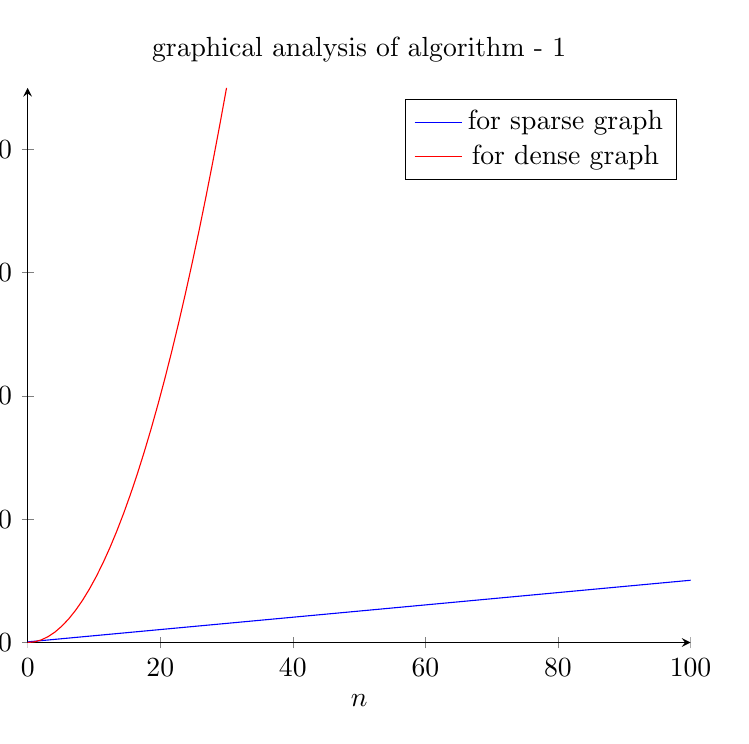
\begin{tikzpicture}[trim left=0cm]
\begin{axis}[
    axis lines = left,
    title=graphical analysis of algorithm - 1,
    xlabel = $n$,
    ylabel = {T},
]
%Here the blue parabloa is defined
\addplot [
    domain=0:100, 
    samples=1000, 
    color=blue,
    ]
    {x+1};
\addlegendentry{for sparse graph}
%Below the red parabola is defined
\addplot [
    domain=0:30, 
    samples=30, 
    color=red,
]
{x^2};
\addlegendentry{for dense graph}
\end{axis}
\end{tikzpicture}

\textbf{Graph 1 :} for sparse graph, no. of edges = $n$, the graph has linear behaviour and for dense graph, no. of edges = $n^2$, the graph is showing quadratic behaviour.

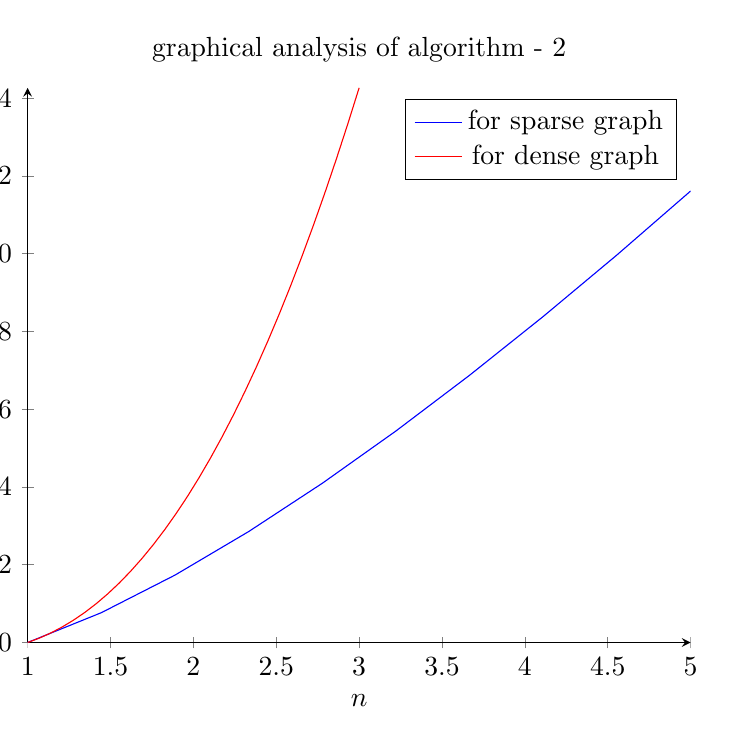
\begin{tikzpicture}[trim left=0cm ]
\begin{axis}[
    axis lines = left,
    title=graphical analysis of algorithm - 2,
    xlabel = $n$,
    ylabel = {T},
]
%Here the blue parabloa is defined
\addplot [
    domain=1:5, 
    samples=10, 
    color=blue,
    ]
    {x*log2(x)};
%     % \addplot[cyan,domain=0.001:4] {abs(log10(x))};
\addlegendentry{for sparse graph}
%Below the red parabola is defined
\addplot [
    domain=1:3, 
    samples=30, 
    color=red,
]
{(x^2)*log2(x)};
\addlegendentry{for dense graph}


\end{axis}
\end{tikzpicture}
\textbf{Graph 2 :} for sparse graph, no. of edges = $n$, the graph has somewhat linear behaviour and for dense graph, no. of edges = $n^2$, the graph is showing somewhat quadratic behaviour.


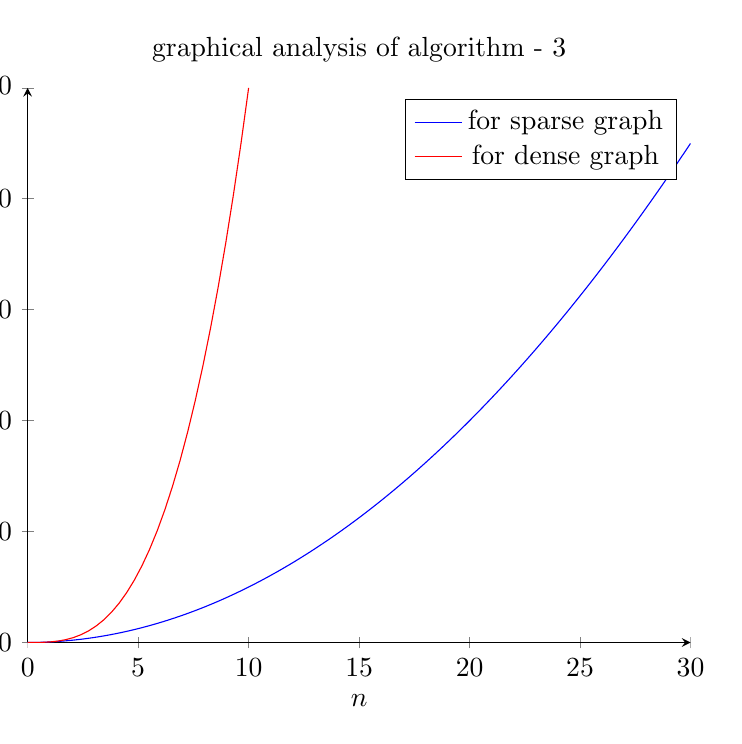
\begin{tikzpicture}[trim left=0cm]
\begin{axis}[
    axis lines = left,
    title=graphical analysis of algorithm - 3,
    xlabel = $n$,
    ylabel = {T},
]
%Here the blue parabloa is defined
\addplot [
    domain=0:30, 
    samples=100, 
    color=blue,
    ]
    {x^2};
\addlegendentry{for sparse graph}
%Below the red parabola is defined
\addplot [
    domain=0:10, 
    samples=30, 
    color=red,
]
{(x^3)};
\addlegendentry{for dense graph}


\end{axis}
\end{tikzpicture}


\textbf{Graph 3 :} for sparse graph, no. of edges = $n$, the graph has quadratic behaviour and for dense graph, no. of edges = $n^2$, the graph is showing somewhat cubic behaviour.

% \textbf{Graph - 2 : } 

% \begin{tikzpicture}
% \begin{axis}[
%     title=graphical behaviour of $O(n+mlogm)$,
%     % hide axis,
%     colormap/cool,
% ]
% \addplot3[
%     mesh,
%     samples=50,
%     domain=-8:8,
% ]
% {x + y*(log2(y))};
% \addlegendentry{$n+mlogm$}
% \end{axis}
% \end{tikzpicture}

% \textbf{Graph - 3 : } 


% \begin{tikzpicture}
% \begin{axis}[
%     title=graphical behaviour of $O(nm)$,
%     % hide axis,
%     colormap/cool,
% ]
% \addplot3[
%     mesh,
%     samples=50,
%     domain=-8:8,
% ]
% {x*y};
% \addlegendentry{$nm$}
% \end{axis}
% \end{tikzpicture}





% \end{thebibliography}
\section{Conclusion\\}
 Here we discussed algorithms to solve SSSP for undirected graph.
For Unweighted graph, the distances can be computed in almost linear time complexity but for weighted graph, there exist several algorithms for different types of graphs.

% \begin{thebibliography}{00}
\section{Reference}
\begin{enumerate}
    \item \url{https://en.wikipedia.org/wiki/Shortest_path_problem}
    \item \url{https://www.tutorialspoint.com/single-source-shortest-paths-arbitrary-weights}
\end{enumerate}


\end{document}


% Intro by gopal, algo by Divyesh, analysis by Akash

